Algoritmi strojnog učenja ovise o dostupnim podacima, ne samo o broju već i kvaliteti.
Metode nadziranog učenja (\emph{eng. Supervised learning}) uz same podatke moraju na raspolaganju imati i oznaku (\emph{eng. Label}) koja definira točno što je svaki podatak prema čemu se uspoređuju i sami izlazi modela.
U puno slučajeva oznake se unose ručno što je dugotrajan i težak proces podložan greškama.
Nenadzirano učenje (\emph{eng. Unsupervised learning}) je privlačno zbog mogućnosti pronalaska i učenja distribucije danih podataka bez potrebe oznaka (\cite{ev_var_ae}).

Generativni modeli osim rješavanja danog problema, tijekom tog procesa \emph{uče} o samim podacima.
Pretpostavka je da podaci nisu u potpunosti nasumični već da dolaze u određenoj distribuciji.
Model se toj distribuciji prilagođava te ima sposobnost generiranja sintetičkih podataka koji joj odgovaraju.
Ovo poglavlje i rad fokusirati će se na model \texttt{autoenkodera}. \\
U nastavku se nalazi detaljnije opisan rad modela, implementacija, rezultati implementacije i poteškoće koje se javljaju.

\section{Autoenkoder}
Autoenkoder je generativni model učen nenadzirano.
Interesantan dio je "skriveni" sloj, najčešće manje dimenzije nego ulazni vektor, iz kojeg dekoder stvara izlaz.
Skriveni sloj sadrži podatke potrebne za uspješnu rekonstrukciju.
Nenadzirano učenje vrši se direktnom usporedbom ulaza i dobivenog konačnog izlaza.
Želja je što vjernije reproducirati ulazne vektore, naravno, uz izbjegavanje direktnog kopiranja.
Direktno kopiranje izbjegava se automatski korištenjem međusloja manje dimenzije prisiljavajući na taj način model da uči iz značajki.

\subsection{Arhitektura}

\begin{figure}[H]
	\centering
	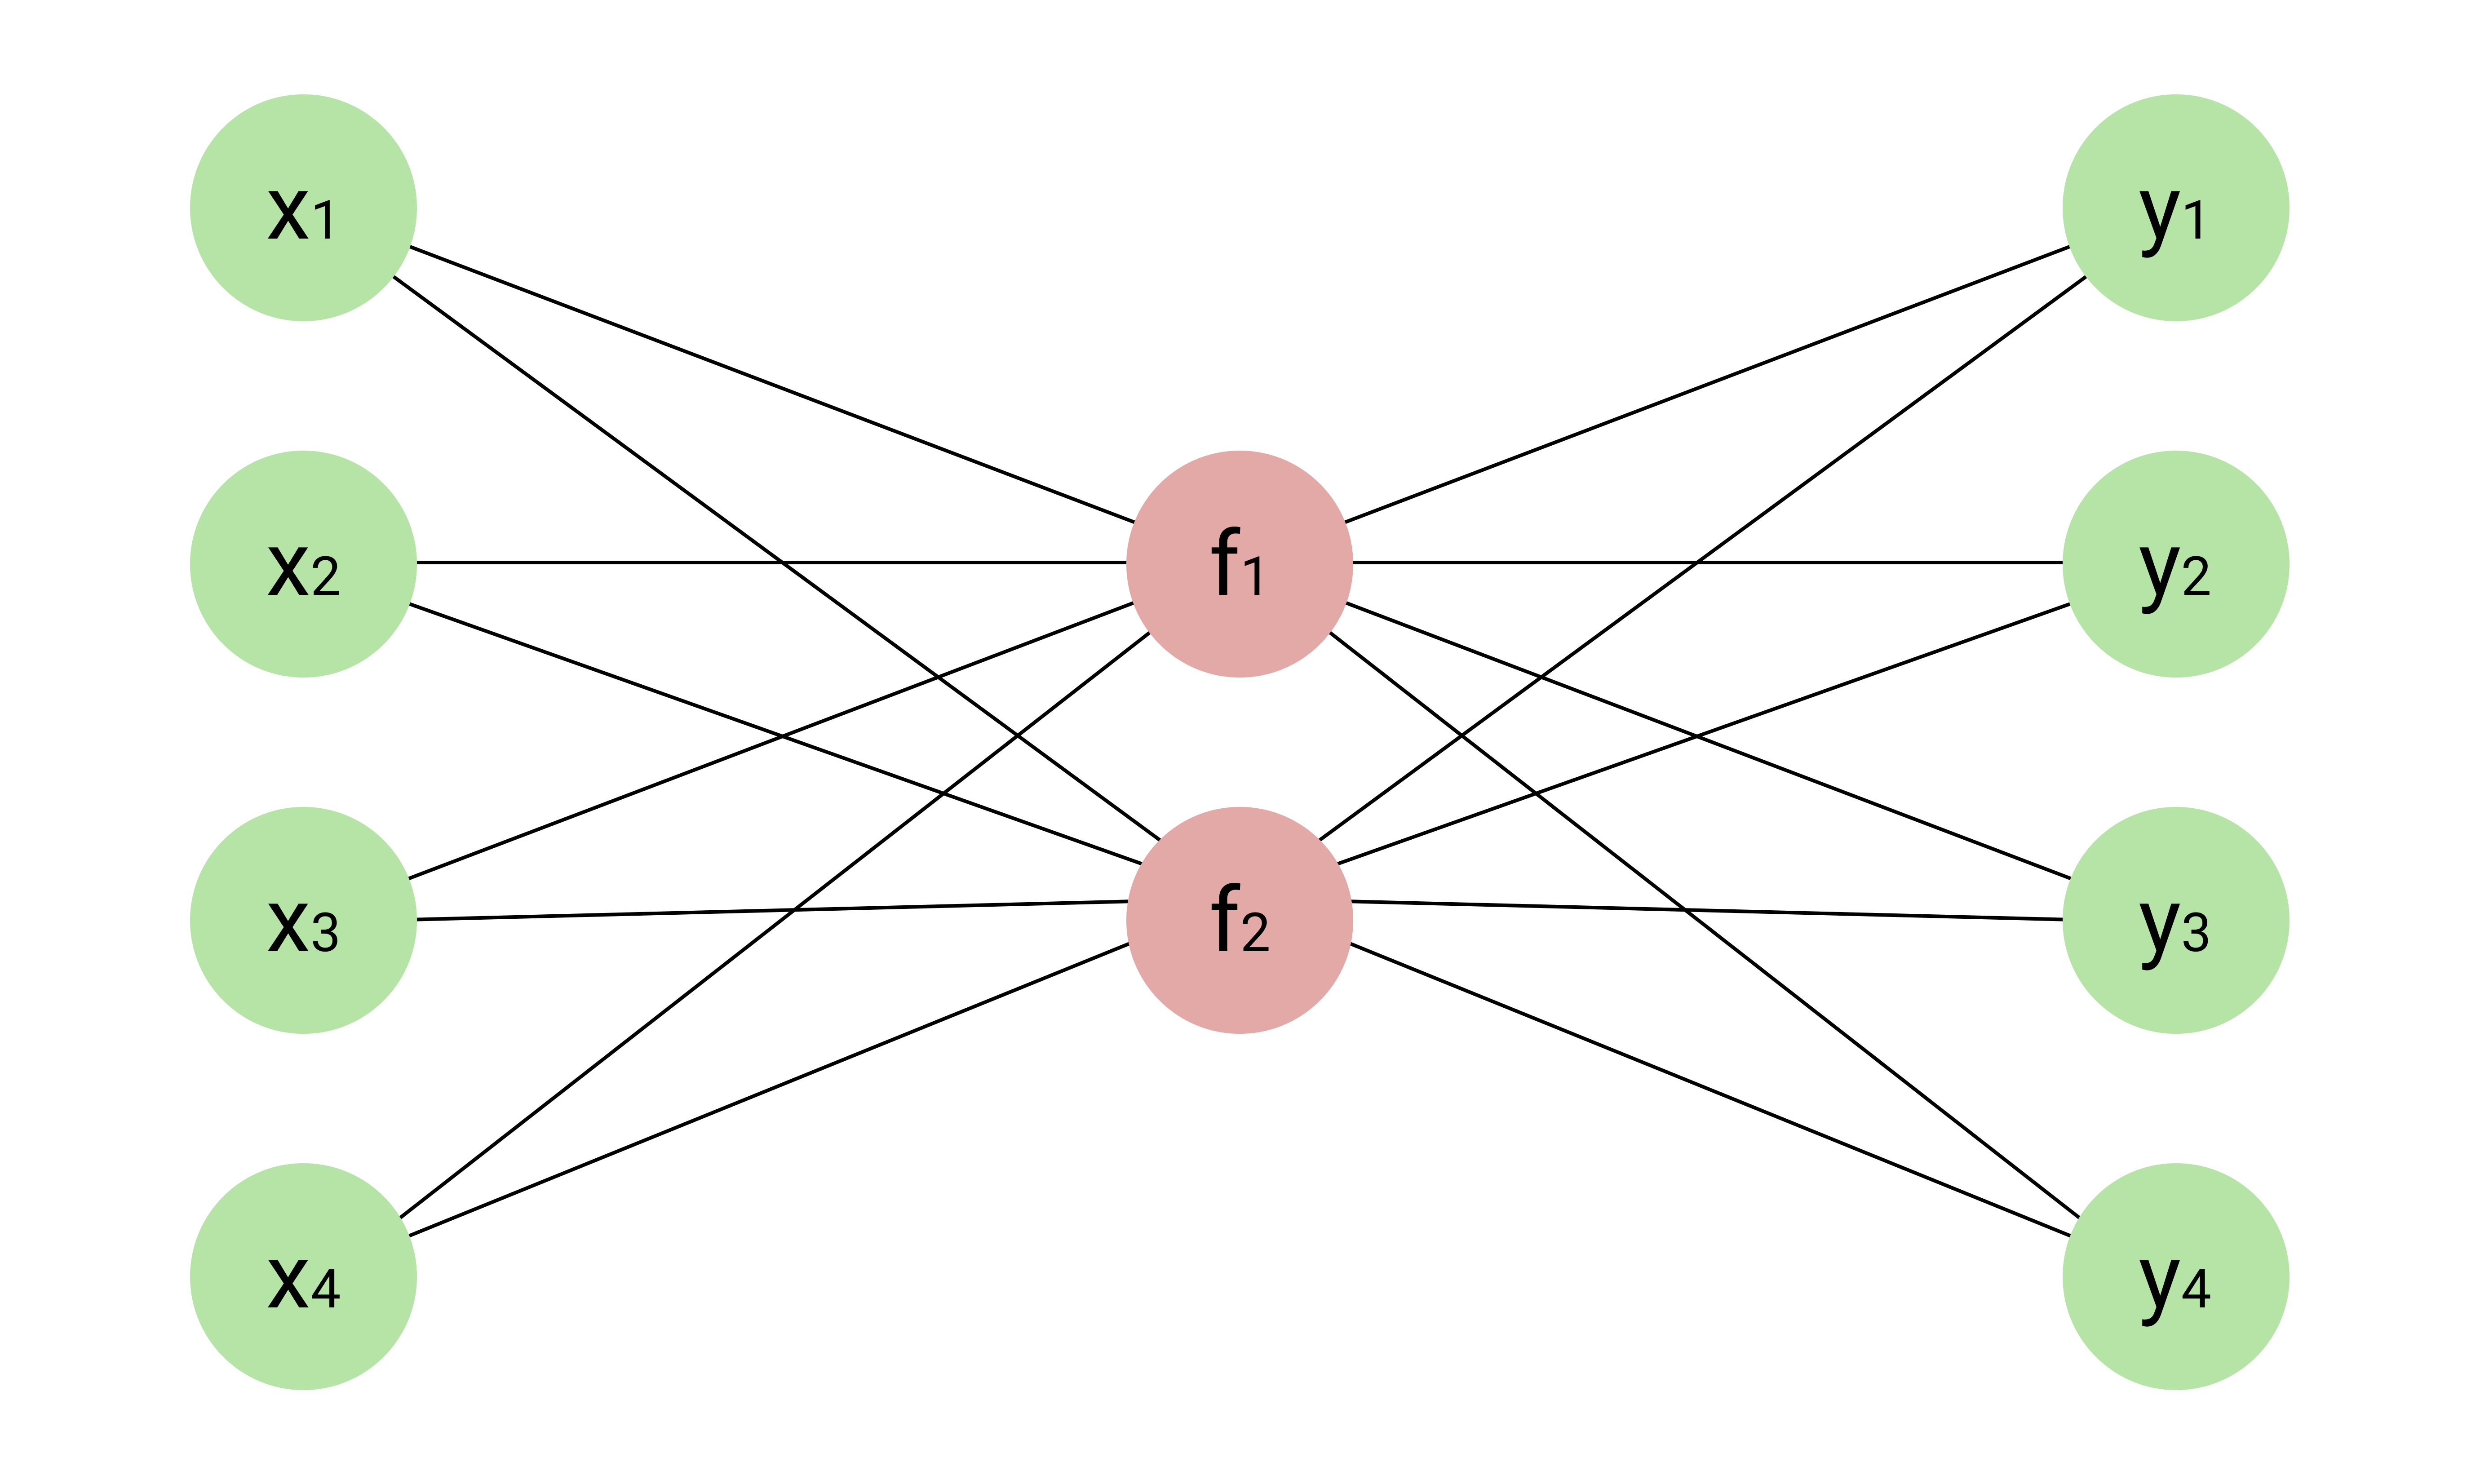
\includegraphics[width=0.8\linewidth]{Illustrations/encoder_example.png}
	\caption{Jednostavan primjer autoenkodera}
	\label{fig:autoencoder_example}
\end{figure}

Pojednostavljena arhitektura autoenkodera vidljiva je na slici \ref{fig:autoencoder_example}.
Izlazni vektor $[y_1 \cdots y_n]$ treba biti što sličniji ulaznom $[x_1 \cdots x_n]$.

\textbf{Enkoder} je prvi dio modela, između ulaza i skrivenog sloja iz ulaza stvara bitne značajke koje mu odgovaraju.
\textbf{Dekoder} iz značajki nastalih od enkodera čini transformaciju do izlaza. \\
Ključ je u srednjem, skrivenom sloju.
Prisiljava model na učenje samo bitnih značajki, redukciju dimenzionalnosti i izbjegavanje direktnog kopiranja.
Konačno, dekoder se može koristiti kao zasebni, generativni model koji iz danih parametara $[f_1 \cdots f_n]$ može generirati izlaz.

\section{Kartezijsko genetsko programiranje za generiranje podataka, CGPAE}
Genetsko programiranje je rijetko korišten alat za probleme koji se rješavaju nenadziranim učenjem.
Po mojim znanjima, ne postoji rad koji koristi Kartezijsko genetsko programiranje za izvedbu autoenkodera.
\cite{why_ae_diff} koristi jednostavan linearni genetski program s više ulaza i izlaza (LGP) umjesto CGP-a.
Smatram da je CGP fleksibilniji i ima veće računalne mogućnosti te pruža veći potencijal za bolje rezultate.
Željeni rezultat je osim uspješnog modela, model koji nosi prednosti genetskog programiranja kao što je čitljivost funkcija koje izvode enkoder i dekoder.

U prijašnjim poglavljima CGP je pokazao dobre rezultate u konvoluciji slike.
Dobre performanse u simboličkoj regresiji su također poznate.
S tim na umu, autoenkoder se čini kao moguć zadatak za riješiti.

\begin{figure}[H]
	\centering
	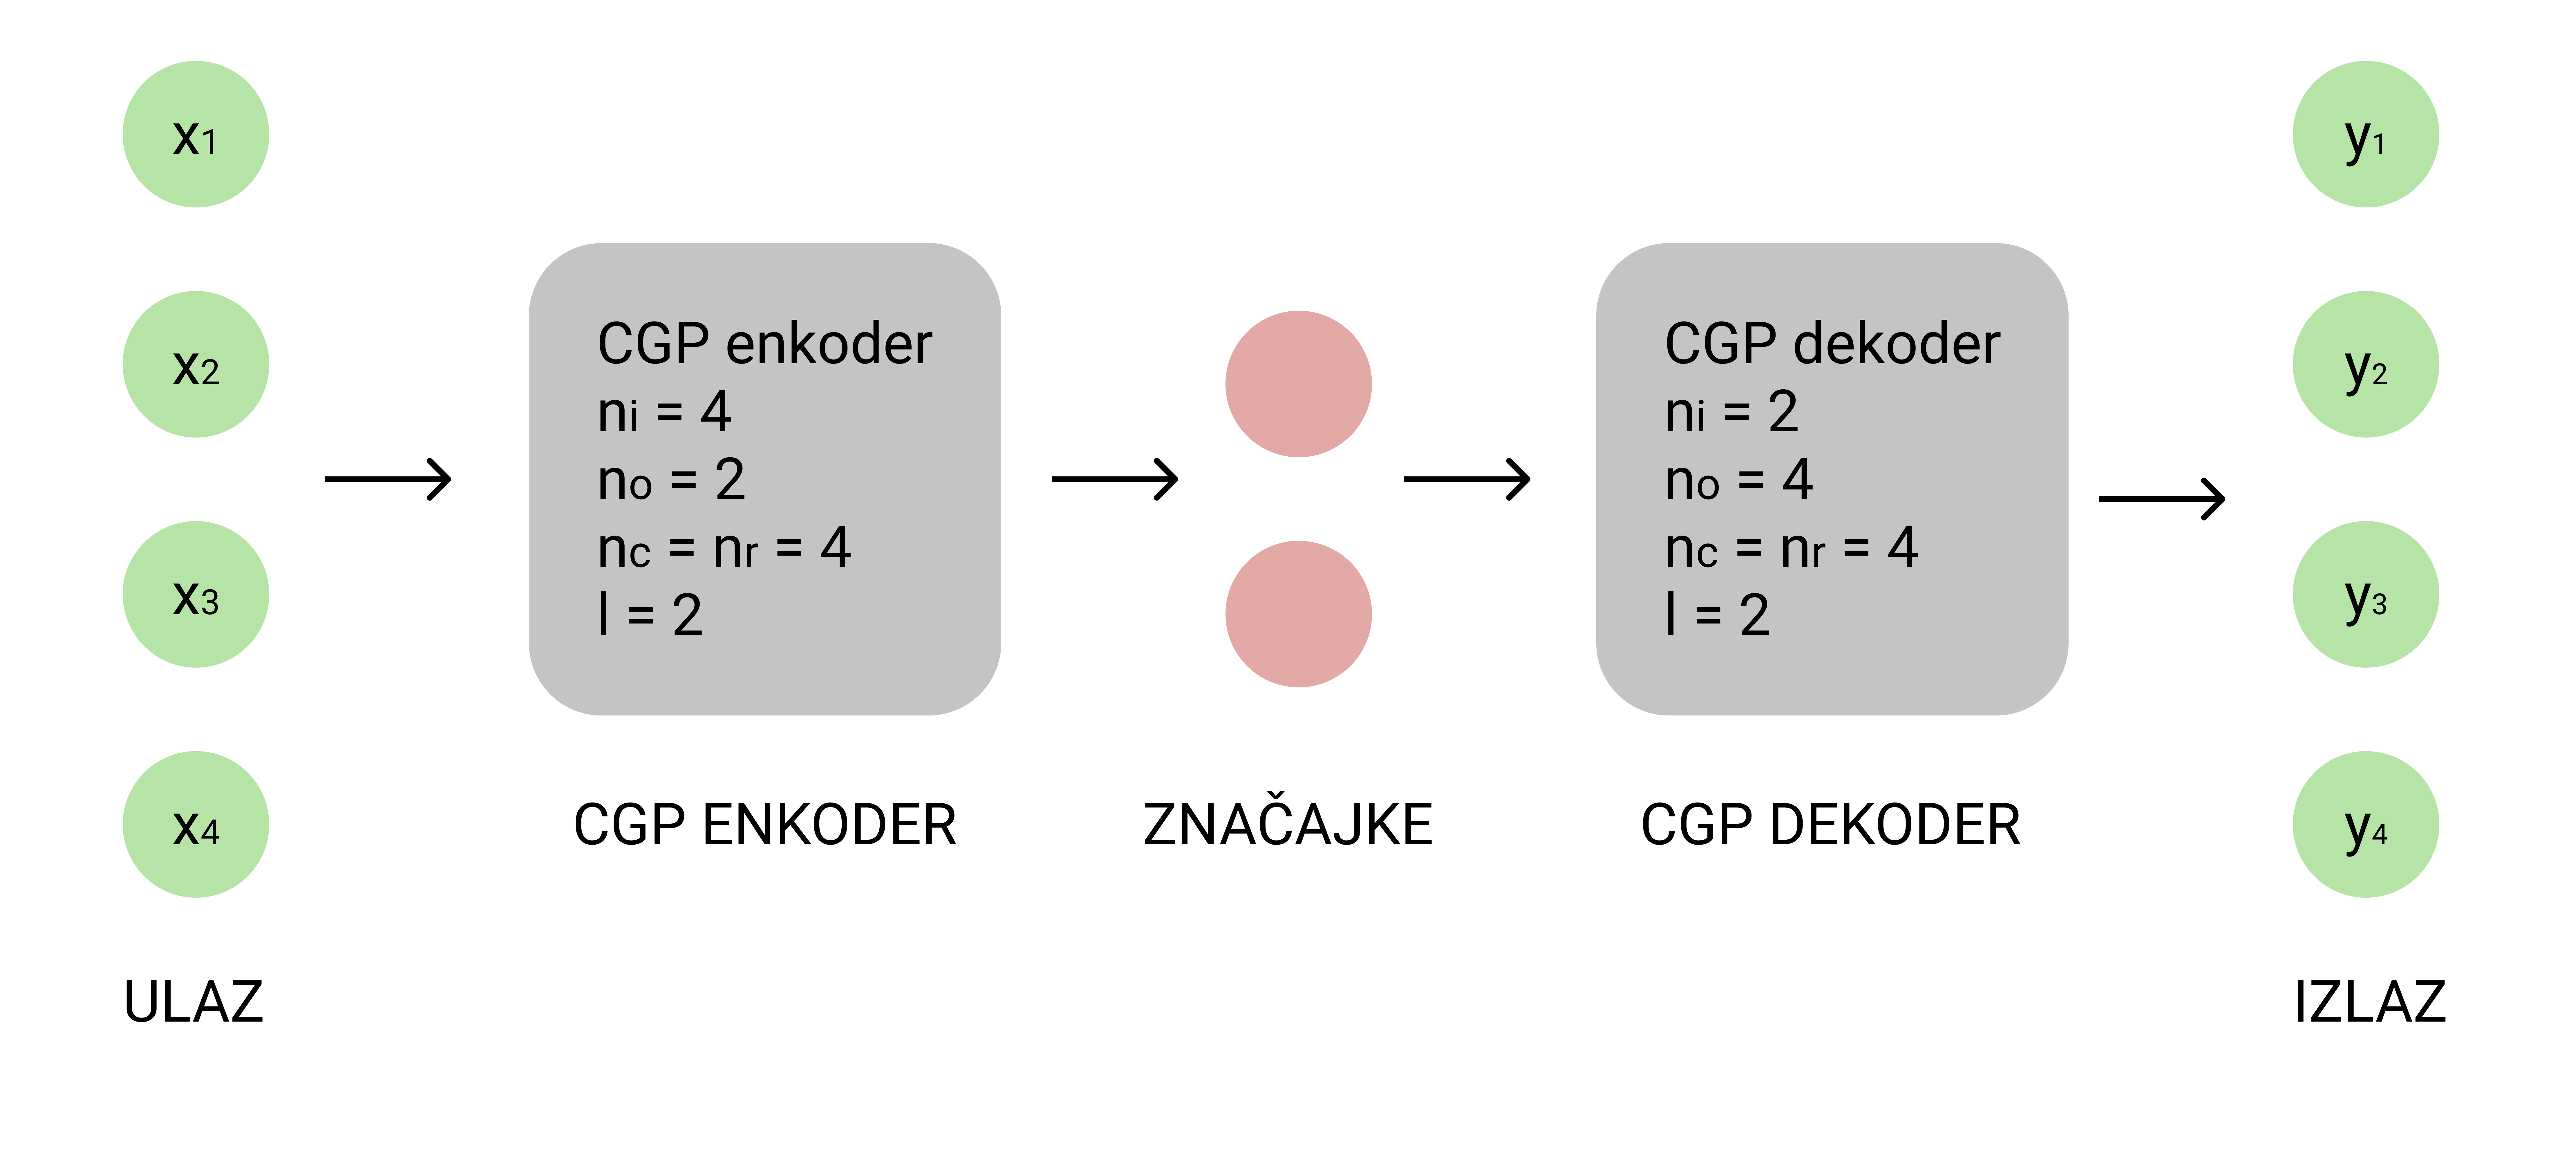
\includegraphics[width=\linewidth]{Illustrations/cgp_encoder_example.png}
	\caption{Prikaz predložene arhitekture \emph{CGPAE}}
	\label{fig:cgpae}
\end{figure}

Slika \ref{fig:cgpae} prikazuje shematiku predložene arhitekture.
Koriste se dva neovisna CGP-a spojena serijski na način da drugi CGP izravno čita izlaz prvog.
Prvi CGP, enkoder, za izlaz stvara vektor veličine po izboru koji sadrži značajke iz ulaza.
Nastavlja se na drugi CGP, dekoder, koji iz vektora značajki stvara izlaz jednakih dimenzija kao ulaz u enkoder.
Njegov izlaz treba biti što sličniji ili isti ulazu u enkoder.

\subsection{Algoritam učenja}
Istovremeno učenje dva odvojena CGP-a predstavlja velik izazov zbog velikog broja parametara koji mogu poprimiti veliku količinu vrijednosti.
Korištenje dva CGP-a može se izbjeći korištenjem jednog s postavljenim $l = 1$.
Ograničenje koje time nastaje je ne-fleksibilnost parametra i postavljanje latentnog vektora značajki na dimenziju jednaku ulazu.
Dva odvojena CGP-a osiguravaju fleksibilnost i dvije različite arhitekture.
Algoritam koji sam koristio inspiriran je serijskom evolucijom koju koristi \cite{conv_gen_programming} gdje $n$ iteracija evoluira svaki sloj pojedinačno prije nego prijeđe na sljedeći.
Algoritam \ref{alg:cgpae_evolution} prikazuje detaljnije provedene korake pri učenju CGPAE sustava.

\begin{algorithm}
	\caption{Algoritam evolucije CGPAE sustava}
	\label{alg:cgpae_evolution}
	\begin{algorithmic}
		\STATE $n \leftarrow broj\ koraka\ prije\ promjene$
		\STATE $cgp\_encoder = stvori\_encoder()$
		\STATE $cgp\_decoder = stvori\_decoder()$
		\STATE $trenirani\_cgp \leftarrow cgp\_encoder$
		\WHILE{uvjet zaustavljanja nije ostvaren}
			\STATE Evaluiraj sustav na skupu podataka
			\STATE Primjeni $1+\lambda$ algoritam na $trenirani\_cgp$

			\IF{napravili $n$ koraka}
				\IF{$trenirani\_cgp = cgp\_encoder$}
					\STATE $trenirani\_cgp = cgp\_decoder$
				\ELSE
					\STATE $trenirani\_cgp = cgp\_encoder$
				\ENDIF
			\ENDIF
		\ENDWHILE
	\end{algorithmic}
\end{algorithm}

\section{Eksperiment}

\begin{figure}[H]
	\centering
	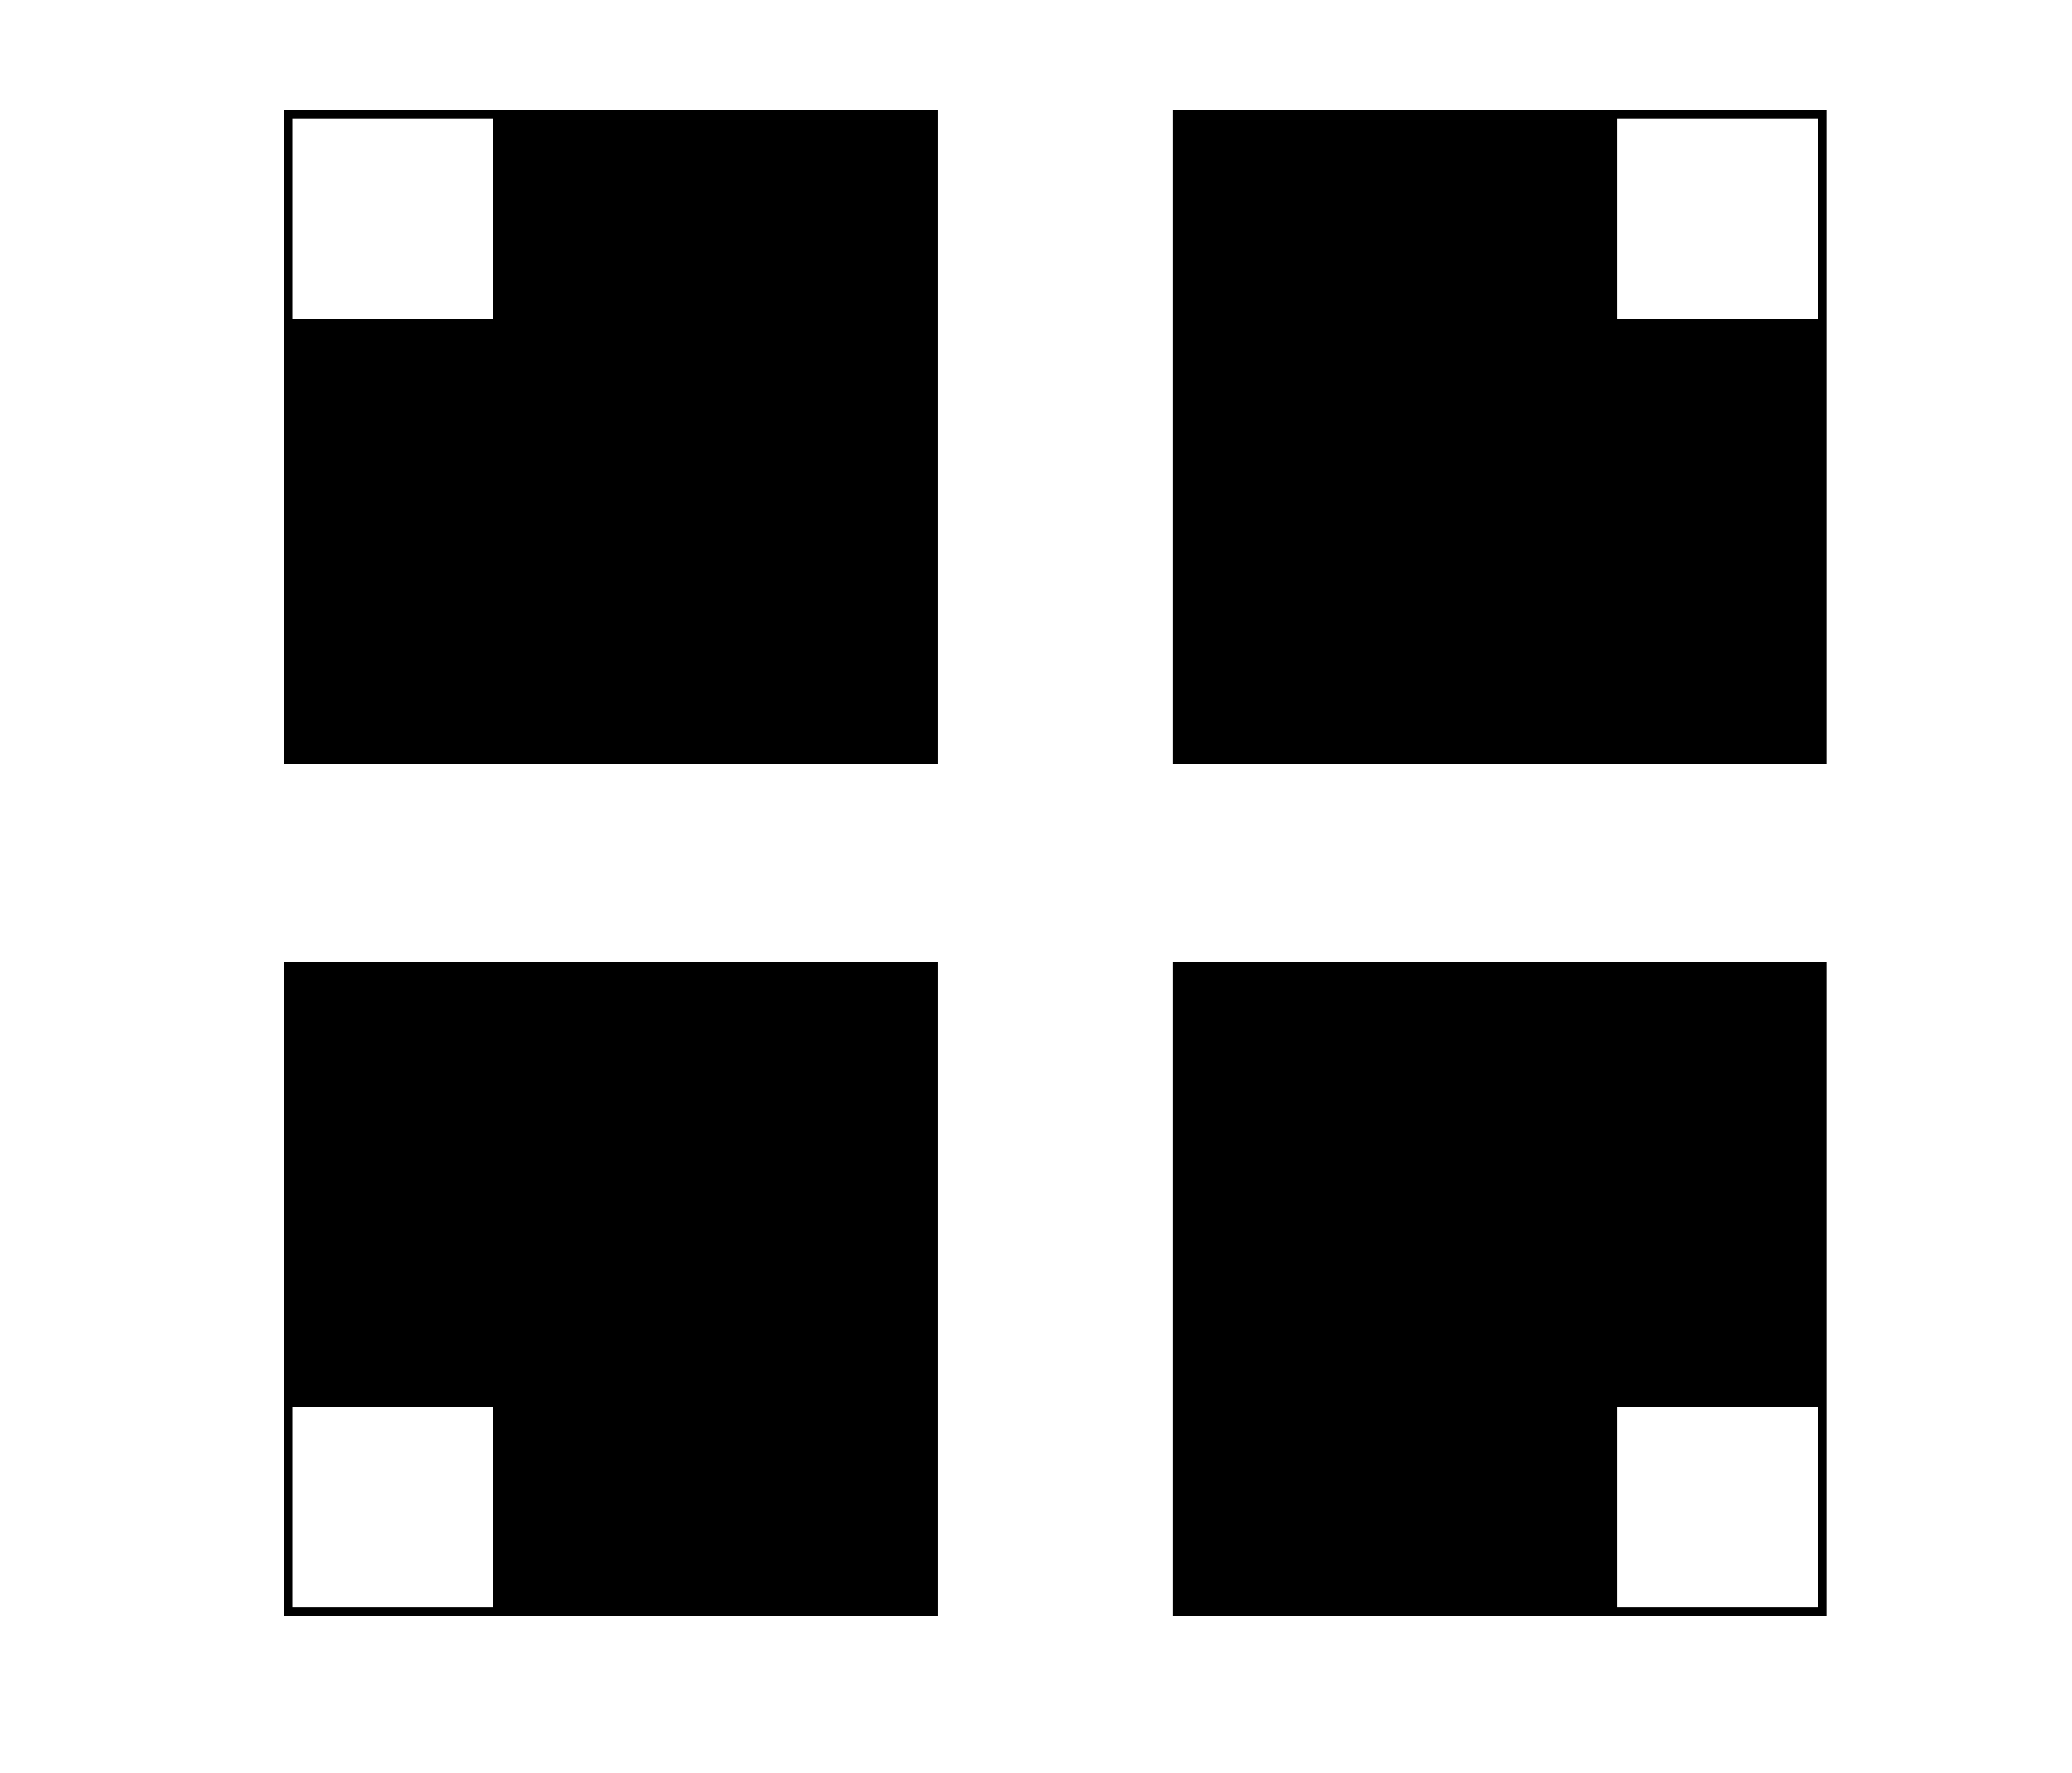
\includegraphics[width=0.6\linewidth]{Illustrations/ae_dataset.png}
	\caption{Grafički prikaz jednostavnog skupa podataka korištenog za ispitivanje CGP-a kao autoenkodera}
	\label{fig:ae_example}
\end{figure}

Za potrebe ispitivanja teze o uspješnosti korištenja CGP-a kao komponente autoenkodera, odlučio sam reproducirati slike veličine $3 \times 3$ vidljive na \ref{fig:ae_example}.
Prilikom ulaska slike u enkoder pretvara se u vektor $v$ gdje je $|v| = 9$.
Zadaća je autoenkodera stvoriti vektor značajki $f$ s $4$ komponente ($|f| = 4$).
Dekoder iz vektora značajki treba reproducirati dani ulaz.

Nažalost, slično kao i kod \cite{why_ae_diff}, rezultati nisu obećavajući.
Prikaz najboljih rezultata vidljiv je na slici \ref{fig:ae_results}.

\begin{figure}[H]
	\centering
	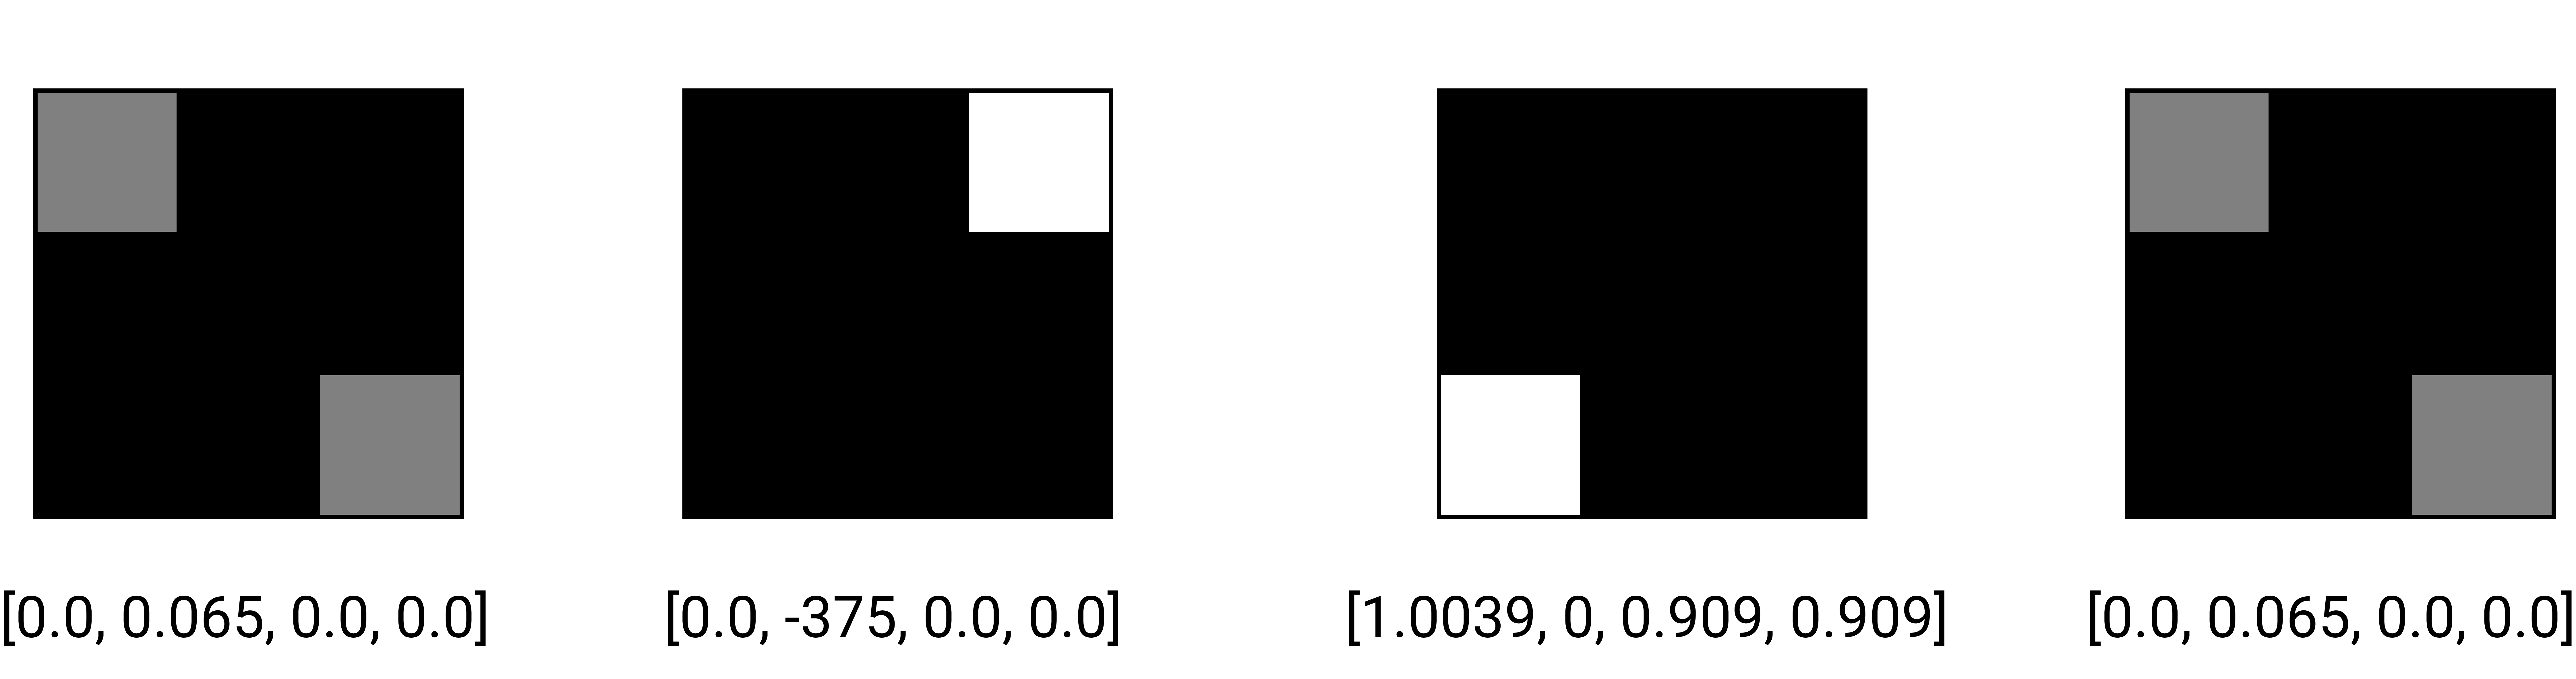
\includegraphics[width=\linewidth]{Illustrations/ae_result.png}
	\caption{Primjer rezultata dobivenih CGPAE modelom. Uz dobivene slike prikazan je i vektor značajki izračunat od enkodera.}
	\label{fig:ae_results}
\end{figure}

Korišteni parametri su sljedeći:
\begin{itemize}
	\item {najviše generacija $\leftarrow 1000$}
	\item {$n = 8$ (Broj koraka između izmjene treniranog CGP-a)}
	\item {Enkoder}
		\subitem {$n_c, n_r = 10, 6$}
		\subitem {$n_i, n_o = 9,4$}
		\subitem {$l = 2$}
		\subitem{$n_{func} = 20$ (Broj raspoloživih funkcija) } 
	\item {Dekoder}
		\subitem {$n_c, n_r = 10, 9$}
		\subitem {$n_i, n_o = 4,9$}
		\subitem {$l = 2$}
		\subitem{$n_{func} = 20$}
\end{itemize}
Ideja je bila početi s jednostavnim skupom podataka (npr. kao na slici \ref{fig:ae_example}) te prelaziti na postupno složenije skupove podataka također korištene u \cite{why_ae_diff}.
No, neuspjeh na jednostavnom skupu podataka doveo je do zaključka da bi složeniji skupovi podataka predstavljali još veći problem.
Uz iste parametre također isproban je jednak skup podataka, no s ulaznim veličinama $2 \times 2$, odnosno, bez praznina između uglova.
CGPAE u tom slučaju lako pronalazi rješenje.
Graf \ref{fig:ae_boxplot} prikazuje ovisnost broja značajki očitanih od enkodera i ukupne pogreške.
Zanimljivo je primijetiti kako broj značajki ne utječe puno na medijan, no najmanji broj, u ovom slučaju $|f| = 2$ ima najmanju vrijednost za odskakajuću pogrešku.

\begin{figure}[H]
	\centering
	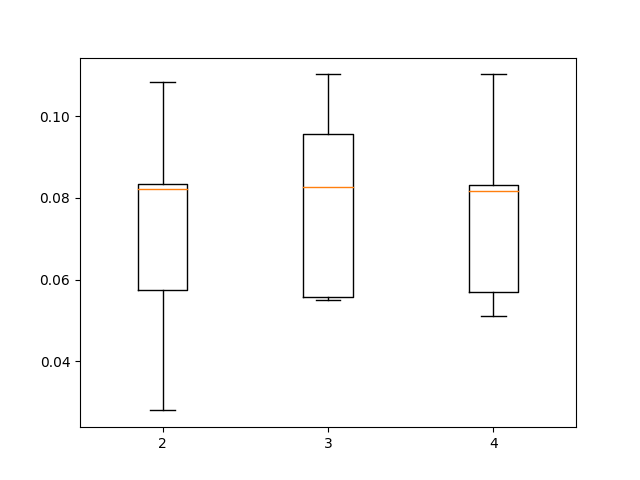
\includegraphics[width=0.6\linewidth]{Illustrations/ae_lat_vec_boxplot.png}
	\caption{Ovisnost broja značajki koje generira enkoder i pogreške tijekom 50 neovisnih pokretanja algoritma}
	\label{fig:ae_boxplot}
\end{figure}
